

The EUTelescope package \cite{Corrin2009} provides software tools for offline analysis and reconstruction of telescope test beam data. 
EUTelescope is embedded into the ILCSoft framework which provides the basic building blocks for offline analysis such as a data model (Linear Collider I/O, \emph{LCIO}),
 a geometry description language (\emph{GEAR}) and the central event processor (\emph{Marlin}) \cite{EUDET-2008-48}. 
EUTelescope comes with its own job submission framework \emph{jobsub} that allows to run analysis jobs locally or to submit them to larger computing clusters such as NAF.

Marlin allows the modular composition of analysis chains for various applications since every task is implemented as an independent \emph{processor} that is called by Marlin. 
The processors expose a set of parameters to the user which can be configured and loaded at runtime via so-called \emph{steering files} in XML format.
This way the Marlin/Processor architecture gives a lot of flexibility to the end user. 

EUTelescope provides several processors for Marlin implementing algorithms necessary for a full track reconstruction and data analysis of beam test experiments. 
Figure~\ref{fig:offline:strategy} shows the analysis strategy of the framework starting from the recorded detector response to the final aligned particle tracks. 
%An overview of the processor range provided by EUTelescope is given in \cite{EUDET-2007-20}.
For low-energy beams such as the DESY-II and ELSA testbeam facilities multiple scattering is the dominating source of track resolution uncertainties. 
Therefore EUTelescope provides advanced algorithms such as General Broken Lines (GBL) \cite{Kleinwort-2012} for tracking which accounts for scattering in all material present in the beam. 
In addition, precise software alignment can be performed using the Millipede-II algorithm \cite{Blobel-2006}.

Support for tracking in presence of magnetic fields and a more fine-grained detector geometry description interface using ROOT::TGeo are currently under development.

\begin{figure}[tbp]
	\center
	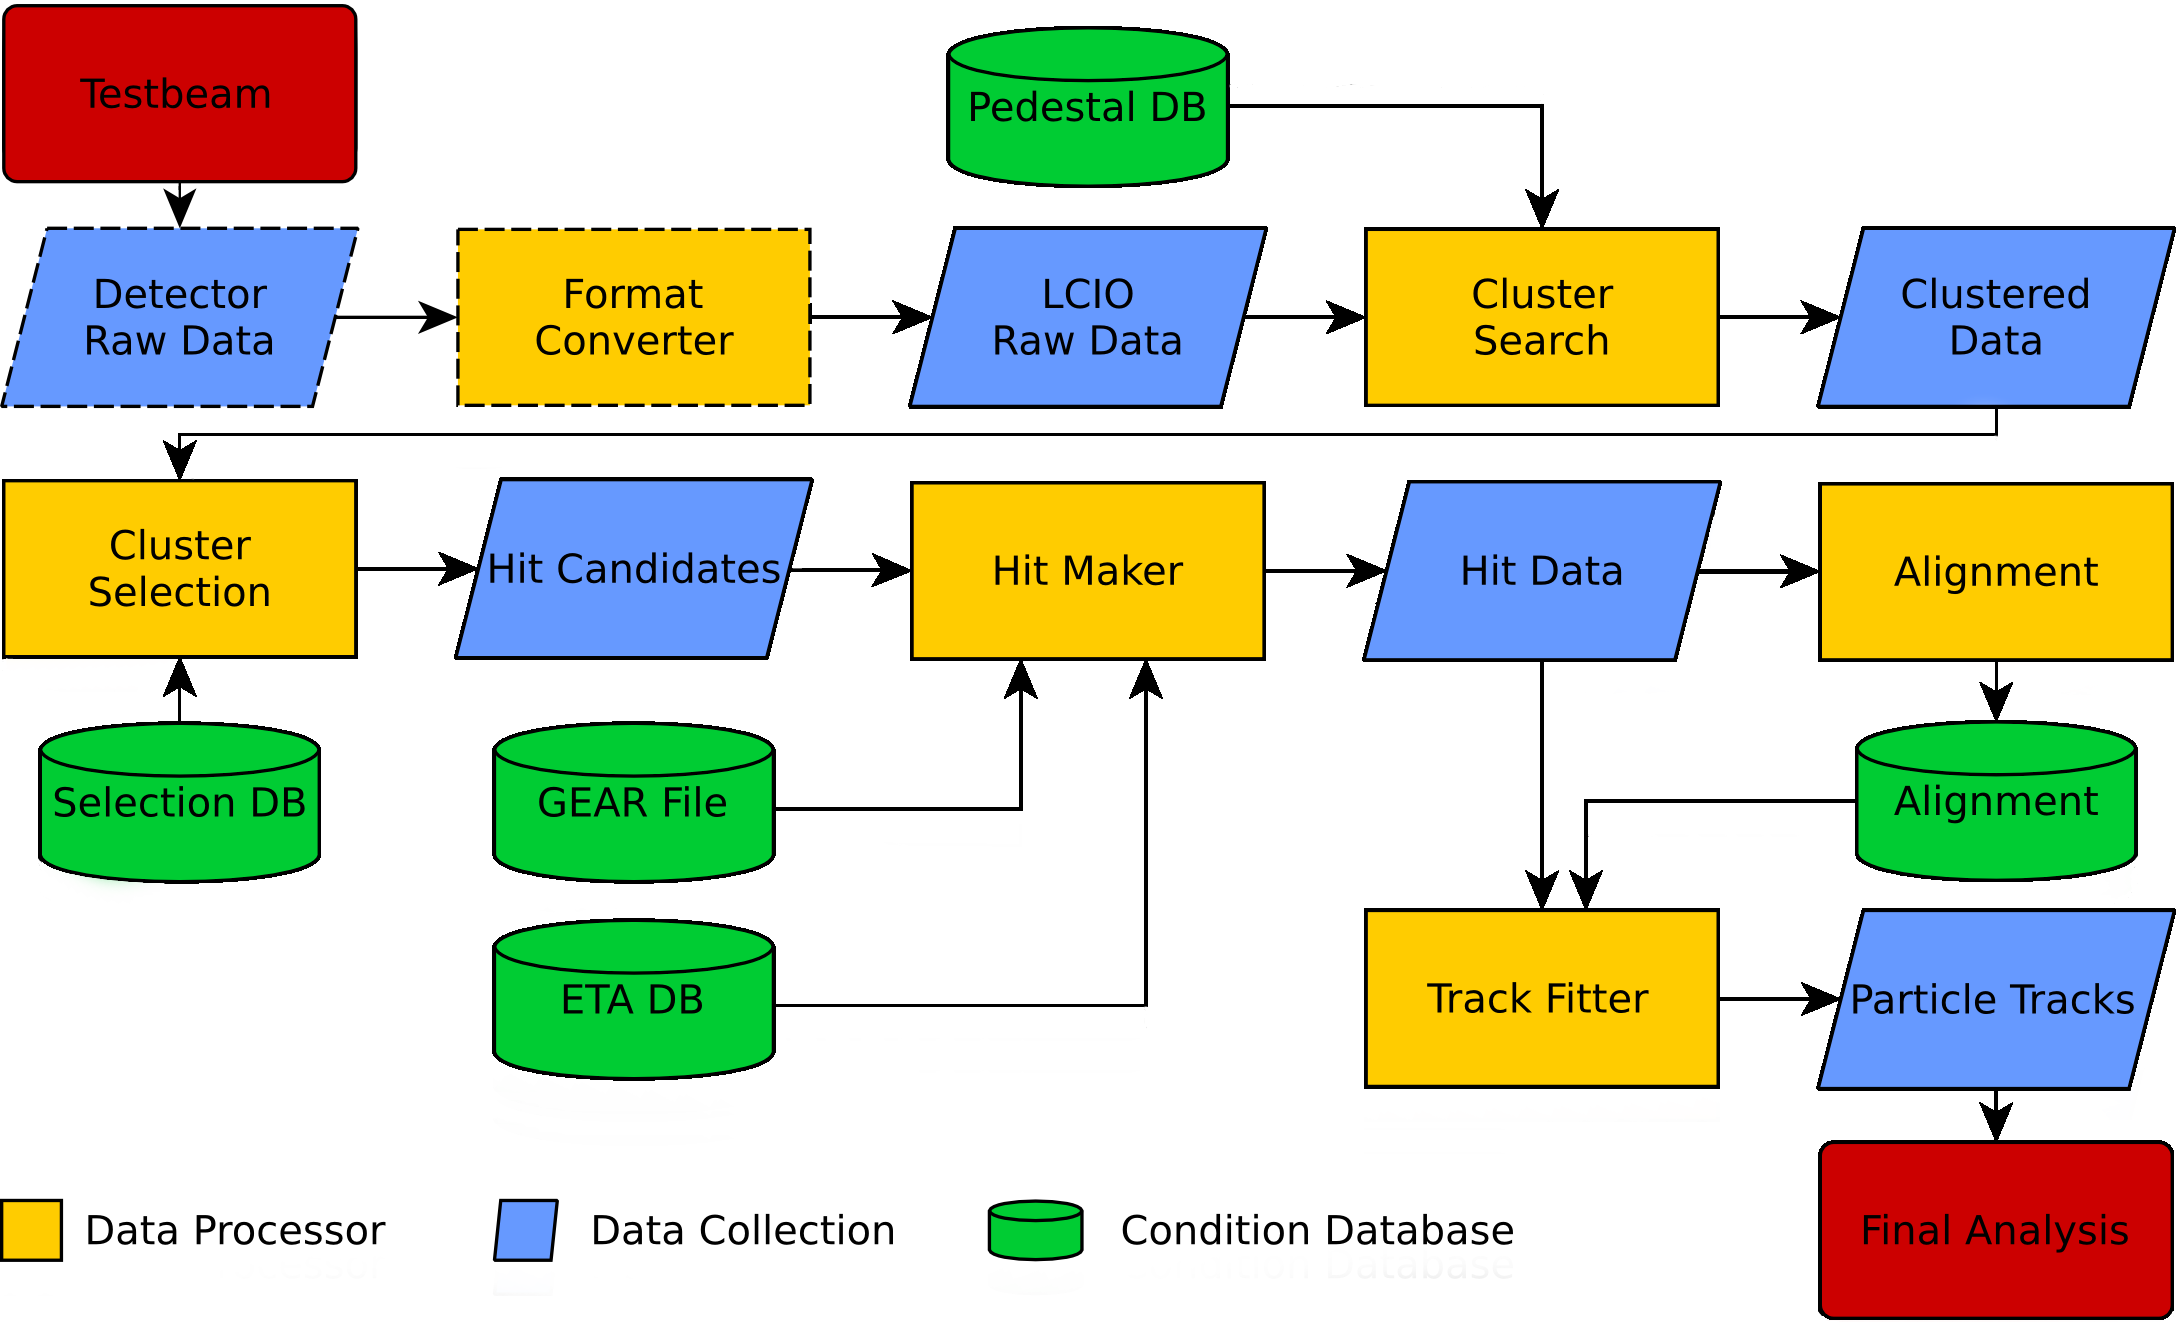
\includegraphics[width=.9\textwidth]{figures/eutel-strategy.png}
	\caption[The EUTelescope data analysis strategy]{Schematic of the overall telescope data reconstruction and analysis strategy of the EUTelescope framework. 
	EUTelescope provides processors for all steps except for the ones with dashed outline; these have to be implemented by the user.}
	\label{fig:offline:strategy}
\end{figure}

\subsection{The \texttt{datura-noDUT} example processors}
\label{sec:datura-nodut}

Within EUTelescope, an example set of processors and configurations were created
as an introduction for new users to EUTelescope. Two GEAR files are provided,
for different telescope geometries. As the name suggests, no external device
under test is used, only the six MIMOSA 26 telescope planes are included. The
goal of the \texttt{datura-noDUT} example is to get from raw detector data to
unbiased track residuals of each telescope plane. A definition of the unbiased
residual distribution will be given in section~\ref{sec:telescoperesolution}. In
the \texttt{datura-noDUT} directory, there are several subdirectories and
configuration files:

\begin{itemize}

\item \texttt{output/} This folder contains all output from EUTelescope. The
LCIO files are stored here, along with log output, \texttt{ROOT} histograms and
alignment constants.

\item \texttt{steering-files/} The steering files are located in this folder.
Each step used within the example has its own steering file containing Marlin
processors.

\item\texttt{config.cfg} In this file all configuration settings are stored.
Global settings, such as the path to the raw data, as well as optional
parameters for the processor steering files are located here.

\item \texttt{runlist.csv} The runlist contains the run numbers of the raw
data and can include parameters for each run, such as geometry used, or
threshold applied, which are passed to the Marlin processor.

\end{itemize}

The \texttt{datura-noDUT} example is constructed such, that a certain sequence
of steering files is called. After all steps have been applied on a run, the
unbiased residuals for this run should have been successfully calculated. An
overview of the steps is shown in figure~\ref{fig:datura-nodutsequence}.

\begin{figure}[tbp]
  \centering
  \includegraphics[width=0.9\textwidth]{figures/datura-noDUT.pdf}
  \caption[Steps performed in the \texttt{datura-noDUT} example]{Sequence of the
steps performed in the \texttt{datura-noDUT} example. Data states are indicated
blue, external files green.}
  \label{fig:datura-nodutsequence}
\end{figure}

The first steering file called is the converter. Its goal is to convert the raw
MIMOSA 26 detector data into the LCIO format and remove any noisy pixels. For
this, it calls two Marlin processors: the \texttt{EUTelNativeReader} and the
\texttt{EUTelAutoPede\-stalNoiseProcessor}.

Following the converter, the clustering is performed. The processor used for
this is \texttt{EUTelClusteringProcessor}. Clusters are searched on each
telescope plane and written to an LCIO collection. A preliminary correlation is
calculated and can be used for debugging purposes.

The \texttt{EUTelHitMaker} processor called in the hitmaker step transforms the
clusters from two-dimensional entities on a telescope plane into hits in a
global three-dimensional frame. A rough pre-alignment is calculated and stored
in a database file.

For the alignment two separate methods are available - either a simple straight
line tracking with \texttt{EUTelMille} or an implementation of the deterministic
annealing filter (DAF) fitter~\cite{ref:daffitter} \texttt{EUTelDafFitter}. In
both cases, the pre-alignment is loaded and applied to the hit data. Tracks are
searched and passed to \texttt{MillepedeII}~\cite{ref:millepede} to determine
the alignment constants. These constants are then stored in another database
file.

The final fitter step calculates the unbiased residual distribution for each
telescope plane with the \texttt{EUTelDUTHistograms} processor. The prealignment
and alignment are loaded and applied to the hit collections. Once again, tracks
are searched, but with one telescope plane considered passive, thus not
contributing to the track fit. Instead, the track is extrapolated to this plane,
and the residual distance to this plane's hits is calculated. This is repeated
for each telescope plane, with histograms written to \texttt{ROOT} files.


